\chapter{Difference-in-Differences}
\label{ch-did}

This chapter is based on
Ref.\cite{book-mixtape}.

This chapter assumes that the
reader has read Chapter \ref{ch-po}
on Potential Outcomes.
DID theory 
applies the basic single-time
PO theory described in Chapter \ref{ch-po}
to 2
well separated times
in which
different conditions prevail.


The Difference-in-Differences (DID)
method was first used by John Snow
in an 1854 report that
argued that 
cholera in London
was being transmitted 
by sewage polluted water
rather than, as others
at the time believed, by air (in fetid vapors
called miasmas).
In general, one can
apply DID to discover 
causal effects in historical data.
By {\bf historical data} (aka a {\bf natural
experiment}. See Ref.\cite{wiki-nat-exp})
we mean data that is collected long
after the treatment (rather than during it)
 and is thus
not  subject to 
active intervention
by the experimenter. 



\section{John Snow, DID  
and a cholera
transmission pathway}


\begin{figure}[h!]
\centering
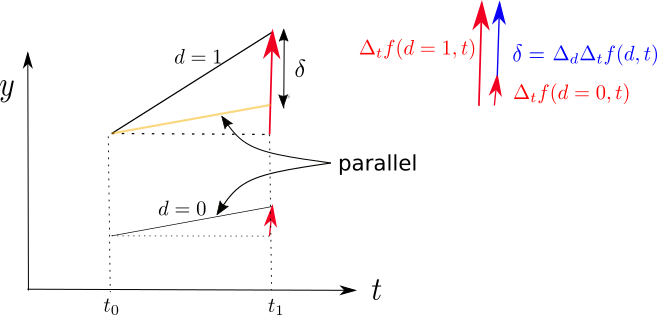
\includegraphics[width=5in]
{did/dif-dif.png}
\caption{Pictorial representation of
 Difference-in-differences (DID) as a difference
of two differences (i.e., 
a difference of two slopes).} 
\label{fig-dif-dif}
\end{figure}

Let

$d\in \bool$

$t\in \{t_0, t_1\}$, $t_0< t_1$

$y=f(d,t)\in \RR$

\beq
\Delta_t f(d,t)= f(d, t_1)-f(d, t_0)
\eeq

\beq
\Delta_d f(d, t)= f(1, t)-f(0, t)
\eeq

\beq
DID=\delta=\Delta_d\Delta_t f(d,t)
\eeq
DID is illustrated in
 Fig.\ref{fig-dif-dif}. 


A {\bf time series} 
is  any function of time
(the domain of the function
is usually a discrete set of times).


In DID, one calculates the slope,
over the same
time interval,
of two time series. One
of the time series ($d=0$)
is for
the control (i.e., untreated) population
and the other ($d=1$) is
 for the treated population.
Then the 
difference $\delta$ of those 2 slopes is taken.
The idea is that if there is no causal difference
between the 2 time series,
then both time
series will 
have the same slope, and
$\delta$ will be zero.

\begin{figure}[h!]
\centering
\includegraphics[width=4in]
{did/did-3-prod}
\caption{$DID=\delta$ expressed as a 
a triple vector product.} 
\label{fig-did-3-prod}
\end{figure}

Note that,
as shown Fig.\ref{fig-did-3-prod},
$DID=\delta$ can also be expressed
as a triple vector product. Indeed,
consider a space
of points $(t, y, z)\in\RR^3$ with
an orthonormal basis
$\hat{t}, \hat{y}, \hat{z}$.
Let $\Delta t = t_1-t_0$.
Let $m_d$ be the slope
of the lines $d\in\bool=
\{$ untreated, treated $\}$. Let

\beq
\vec{r}_d=
(\Delta t,m_d  \Delta t, 0)
\eeq
for $d\in\bool$.
 Then
 
\beqa
\frac{1}{\Delta t}
\vec{r}_0\times \vec{r}_1\cdot \hat{z}
&=&
\frac{1}{\Delta t}
\det
\left[
\begin{array}{ccc}
\Delta t&m_0\Delta t& 0
\\
\Delta t&m_1\Delta t& 0
\\0&0&1
\end{array}
\right]
\\
&=&
(m_1-m_0)\Delta t 
\\
&=& \delta
\eeqa


\begin{table}[h!]
\centering
{\renewcommand{\arraystretch}{1.4}
\begin{tabular}{|c|c|c|}
\hline 
\rowcolor[HTML]{ECF4FF} 
 & $t=t_0 $ (1849) & $t=t_1$$\}$ (1854) \\ 
\hline
$\td=1 $ (town 1)\cellcolor[HTML]{ECF4FF}
&85 deaths, polluted DW&19 death, unpolluted DW\\
\hline 
$\td=0 $ (town 0)\cellcolor[HTML]{ECF4FF} 
&135 deaths, polluted DW& 147 deaths, polluted DW\\ 
\end{tabular}
}
\caption{A condensation of the data
collected by 
John Snow in 1854,
to test the hypothesis
that cholera in London was being spread by
polluted drinking water (DW).}
\label{tab-john-snow}
\end{table}

A condensation of the
data collected by John Snow in 1854
is given in Table \ref{tab-john-snow}.
From that data, we find that

\beq
\delta= \Delta_d\Delta_t f(d,t)=(19-85)-(147-135)=
-66-12=-78
\eeq



\section{PO analysis}
In this section,
we show how
to analyze
DID 
using the formalism of PO theory.

We will speak of a treatment 
outcome
$\rvy^\s(\rvtd, x^\s; t, g^\s)$
for individual $\s$
that depends, not 
just on the treatment dose $\td^\s\in \bool$
and the confounder state $x^\s$,
but also
on a group parameter (i.e., which population
or town)
$g^\s\in \bool$
and on a time parameter $t\in\{t_0, t_1\}$ 
(note $t$ is independent of $\s$).
Actually,
we will assume $g^\s=\td^\s$,
so we will just speak of
$\rvy^\s(\rvtd, x^\s; t)$
with no explicit $g^\s$
dependence. As usual for PO theory,
we will consider
expected values of $y^\s$:


\beq
E_{\s|d,\td, x}[y^\s(\td^\s, x^\s; t)]=
 E_{y|d, \td, x}[\rvy(\td, x; t)]=
\caly_{d|\td, x}(t)
\eeq

To calculate these
expected values, we need a ``model"
with probability 
distributions.
In this case,
the needed model and probability
distributions are
provided by the
bnets depicted in Fig.\ref{fig-did-G-im}.
The TPMs,
printed in blue,
for the 
two bnets
$G(t_0)$
and $G(t_1)$ shown
in Fig.\ref{fig-did-G-im},
are as follows.
Note
that the
TPMs for the
bnets $G(t_0)$
and $G(t_1)$
are defined in 
terms
of the TPMs for the bnet $G$.


\begin{figure}[h!]
$$
\begin{array}{ccccc}
\xymatrix{
&\rvx^\s\ar[dl]\ar[dr]
\\
\rvd^\s\ar[rr]&&\rvy^\s
}
&&
\xymatrix{
&\rvx^\s\ar[dl]\ar[dr]
\\
\rvd^\s=0&\rvtd^\s=\td^\s\ar[r]&\rvy^\s
}
&&
\xymatrix{
&\rvx^\s\ar[dl]\ar[dr]
\\
\rvd^\s=\td^\s&\rvtd^\s=\td^\s\ar[r]&\rvy^\s
}
\\
\\
G&&G(t_0)= \left.G_{im}\right|_{d^\s=0}
&&
G(t_1)=
\left. G_{im}\right|_{d^\s=\td^\s}
\end{array}
$$
\caption{Bnet 
$G_{im}= \kappa_{\rvd^\s\rarrow\rvy^\s}
(\td^\s)G$
is obtained by applying 
the imagine operator to arrow 
$\rvd^\s\rarrow\rvy^\s$
of bnet $G$. Bnet $ G_{im}(t_0)$
is obtained
by setting $\rvd^\s=0$ in bnet $G_{im}$.
Bnet $ G_{im}(t_1)$
is obtained
by setting $\rvtd^\s=\rvd^\s$ in bnet $G_{im}$.
} 
\label{fig-did-G-im}
\end{figure}

\beq\color{blue}
P(x^\s)=P_\rvx(x^\s)
\eeq

\beq\color{blue}
P(d^\s|x^\s)= 
\left\{
\begin{array}{ll}
P_{\rvd|\rvx}(d^\s|x^\s)\delta(d^\s,0)
& \text{ for graph } G(t_0)
\\
P_{\rvd|\rvx}(d^\s|x^\s)\delta(d^\s,\td^\s)
& \text{ for graph } G(t_1)
\end{array}
\right.
\eeq
 
\beq\color{blue}
P(y^\s|\td^\s, x^\s)=
P_{\rvy|\rvtd, \rvx}(y^\s|\td^\s, x^\s)
\eeq

\beq\color{blue}
P((\td^\s)')=\delta(
(\td^\s)', \td^\s)
\eeq

\begin{figure}[h!]
\centering
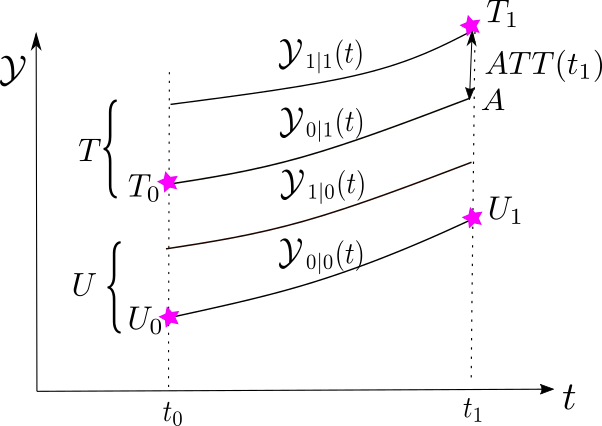
\includegraphics[width=3in]
{did/dif-dif-bc.png}
\caption{
Four different time-dependent
expected 
values $\caly_{d|\td}(t)$ of $y^\s$.
Bnets $G(t_0)$
and $G(t_1)$
are  defined in Fig.\ref{fig-dif-dif}.
The $\caly$ coordinates of the
2 magenta  stars at time
$t=t_0$ (resp., $t=t_1$)
can be calculated using bnet $G(t_0)$
(resp., $G(t_1)$).
} 
\label{fig-dif-dif-bc}
\end{figure}

Henceforth, 
for simplicity, we will
omit the confounder state $x$
from the indices of $\caly$; i.e., we will write
$\caly_{d|\td}(t)$
instead of $\caly_{d|\td, x}(t)$.
The fact that we will
not explicitly
mention $x$ does not
mean that it doesn't exist
or that it doesn't affect our analysis.
John Snow
does not seem to have considered any confounders
in his cholera study,
or else he tried to collect 
data restricted to a single stratum $x$.
If there are confounders,
they cannot be neglected.
As discussed in Chapter \ref{ch-po}
under the subject of strata-matching in PO,
one must condition $\caly$
on a single $x$ stratum
and, later on,  one must average
over all the possible $x$ strata.


Let $\calm\caly_{d|\td}(t)$ denote the
{\bf measured $\caly_{d|\td}(t)$}.
We define this quantity as

\beqa
\calm\caly_{d|\td}(t)
&=&
\left\{
\begin{array}{ll}
\caly_{0|\td}(t) \indi(d=0) 
& \text{ if } t=t_0
\\
\caly_{\td|\td}(t)\indi(d=\td)
 & \text{ if } t=t_1
\end{array}
\right.
\\
&=&
\caly_{0|\td}(t) \indi(d=0, t=t_0)+
\caly_{\td|\td}(t)\indi(d=\td, t=t_1)
\eeqa
Now we claim that the DID 
$\delta$ calculated in the 
previous section for
John Snow's data,
can be expressed in PO formalism as follows:

\beq
\delta=
\Delta_\td\Delta_t \sum_d 
\calm\caly_{d|\td}(t)
\;.
\eeq
Fig.\ref{fig-dif-dif-bc}
depicts the
four functions
$\caly_{d|\td}(t)$
for $t$ in the interval  $[t_0, t_1]$
and for $d,\td\in \bool$.
The $\caly$ coordinates
of the four magenta stars in 
Fig.\ref{fig-dif-dif-bc} can 
be calculated using bnets $G(t_0)$
and $G(t_1)$.

Define
the {\bf parallel trends} (PT)
by 

\beq
PT=\Delta_\td\Delta_t\caly_{0|\td}(t)
\;.
\eeq
We will say the 
{\bf parallel trends assumption (PTA)}
holds if $PT=0$.

Next we prove that
the DID $\delta$ equals
the sum of an ATT\footnote{ATT stands for 
the average treatment effect
of the treated. ATT is defined 
in Chapter \ref{ch-po}} 
and PT.

\beqa
\delta&=&
\Delta_\td\Delta_t \sum_d 
\calm\caly_{d|\td}(t)
\\
&=&\sum_d 
\left[
\Delta_t \calm\caly_{d|1}(t)
-\Delta_t \calm\caly_{d|0}(t)
\right]
\\
&=&\sum_d 
\left[
\calm\caly_{d|1}(t_1)
-
\calm\caly_{d|1}(t_0)
\right]
-\sum_d\left[
\Delta_t \calm\caly_{d|0}(t_1)
-
\Delta_t \calm\caly_{d|0}(t_0)
\right]
\\
&=&
\caly_{1|1}(t_1)-\caly_{0|1}(t_0)
-\{
\caly_{0|0}(t_1)-\caly_{0|0}(t_0)
\}
\\
&=&
\caly_{1|1}(t_1)-\caly_{0|1}(t_0)
-\{
\caly_{0|0}(t_1)-\caly_{0|0}(t_0)
\}
+\underbrace{
\{
\caly_{0|1}(t_1)-
\caly_{0|1}(t_1)
\}}_{\text{ zero }}
\\
&=&
\underbrace{
\caly_{1|1}(t_1) - \caly_{0|1}(t_1)}
_{ATT(t_1)}
-\caly_{0|1}(t_0)
-\{
\caly_{0|0}(t_1)-\caly_{0|0}(t_0)
\}
 + \caly_{0|1}(t_1)
\\
&=&
ATT(t_1)
-\Delta_t \caly_{0|0}(t)
+\Delta_t \caly_{0|1}(t)
\\
&=&
ATT(t_1)
+
\underbrace{\Delta_\td\Delta_t\caly_{0|\td}(t)}_
{\text{ zero if PTA holds}}
\eeqa





\section{Linear Regression}
In this
section,
we show how to apply
linear regression (LR)
to the PO analysis of DID.


As before, let
$y^\s$ be the treatment outcome
for individual $\s$,
who receives
a treatment dose
$\td^\s$
at times $t\in\{t_0, t_1\}$.
$y^\s(\td^\s;t)$
can be fitted as follows.
Here $\eps^\s$
is the residual
for individual $\s$
and $b_0, m_0, b_1, m_1\in \RR$
are the fit parameters.

%
\beq
y^\s = [b_0 + m_0 t](1-\td^\s)
+  [b_1 + m_1 t]\td^\s
+ \eps^\s
\;.
\label{eq-did-lr}
\eeq  
Note that Eq.(\ref{eq-did-lr})
 yields a straight line
in the $y^\s-t$ plane
for $d^\s=0$,
and another 
straight line for $d^\s=1$.
We are
using the
standard symbols
$b$ to denote
the y-intercept, and $m$ 
to denote the slope
of a straight line.

Taking the expected value
of Eq.(\ref{eq-did-lr}), we get

\beq
\caly_{d|\td}(t) = 
[b_0 + m_0 t](1-\td)
+  [b_1 + m_1 t]\td
\;.
\eeq  
with $d=0$ for $t=t_0$
and $d=\td$ for $t=t_1$.

Let $T=t_1-t_0$. Since
$\Delta_t t=T$ and $\Delta_d d=1$, one gets

\beq
\delta=\Delta_d\Delta_t \calm\caly_{d|\td}(t)=
\Delta_d\Delta_t y^\s=(m_1-m_0)T
\;.
\eeq



\begin{figure}[h!]
\centering
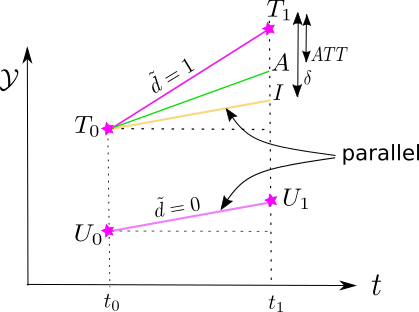
\includegraphics[width=3.5in]
{did/parallel-trends.png}
\caption{We use
Linear Regression
to fit a straight line
between points $S_0$
and $F_0$,
and between points
$S_1$ and $F_1$.
(S=starting, F=finishing).
The $\caly$
coordinates
of $S_0, S_1, F_0, F_1$
are given by Table \ref{tab-did-points}.
The $\caly$
coordinates of points
$I$ (image of point $F_0$)
and $C$ (counterfactual point)
are 
given by Eqs.(\ref{eq-c-i-pts}).
} 
\label{fig-parallel-trends}
\end{figure}

\begin{table}[h!]
\centering
{\renewcommand{\arraystretch}{1.2}
\begin{tabular}{|c|c|c|}
\hline 
\rowcolor[HTML]{ECF4FF} 
 & $t=t_0$ & $t=t_1$ \\ 
\hline
$\td=1$ \cellcolor[HTML]{ECF4FF}& $\caly(S_1)=\caly_{0|1}(t_0)$ & $\caly(F_1)=\caly_{1|1}(t_1)$ \\ 
\hline 
$\td=0$\cellcolor[HTML]{ECF4FF} & $\caly(S_0)=\caly_{0|0}(t_0)$ & $\caly(F_0)=\caly_{0|0}(t_1)$ \\ 
\hline 
\end{tabular}
}
\caption{
$\caly$ coordinates
of points
$S_0, S_1, F_0, F_1$
in Figs.\ref{fig-dif-dif-bc}
 and \ref{fig-parallel-trends}.
}
\label{tab-did-points}
\end{table}



Figs.\ref{fig-dif-dif-bc} and
\ref{fig-parallel-trends}
define
points $S_0, S_1, F_0, F_1, I, C$.
The $\caly$
coordinates of points 
$S_0, S_1, F_0, F_1$ are 
given by
Table \ref{tab-did-points}.
The $\caly$
coordinates of points $C,I$
are given by Eqs.\ref{eq-c-i-pts}.

\begin{subequations}
\label{eq-c-i-pts}
\beq
\caly(C)= \caly_{0|1}(t_1)
\eeq

\beq
\caly(I)=\caly(F_0) + 
[\caly(S_1)-\caly(S_0)]
\eeq
\end{subequations}

We can express $ATT$
and the $\delta$ for DID 
in terms of 
the $\caly$
of the points
$S_0, S_1, F_0, F_1, I, C$. Indeed,

\beqa
\delta&=&\caly(F_1)-\caly(I)
\\
&=&
\caly(F_1)-
\caly(F_0) -
[\caly(S_1)-\caly(S_0)]
\eeqa

\beq
ATT = \caly(F_1)-\caly(C)
\eeq
Hence, 

\beq
\delta=ATT\iff \caly(I)=\caly(C) \iff 
\text{PTA holds}
\eeq